\documentclass[fontset=none]{ctexart}

\usepackage[T1]{fontenc}
\usepackage{fontspec}
\setCJKmainfont{SimSun}
% Latin Modern
\renewcommand*\ttdefault{txtt} % 改等宽字体

\setcounter{tocdepth}{5}
\setcounter{secnumdepth}{5}
% -1 part
% 0 chapter
% 1 section
% 2 subsection
% 3 subsubsection
% 4 paragraph
% 5 subparagraph

\usepackage{cite}
\usepackage{geometry}
\geometry{a4paper,scale=0.8}

\usepackage{algorithm}  
\usepackage{algorithmicx}  
\usepackage{algpseudocode}
\makeatletter
\newenvironment{breakablealgorithm}
  {% \begin{breakablealgorithm}
   \begin{center}
     \refstepcounter{algorithm}% New algorithm
     \hrule height.8pt depth0pt \kern2pt% \@fs@pre for \@fs@ruled
     \renewcommand{\caption}[2][\relax]{% Make a new \caption
       {\raggedright\textbf{\ALG@name~\thealgorithm} ##2\par}%
       \ifx\relax##1\relax % #1 is \relax
         \addcontentsline{loa}{algorithm}{\protect\numberline{\thealgorithm}##2}%
       \else % #1 is not \relax
         \addcontentsline{loa}{algorithm}{\protect\numberline{\thealgorithm}##1}%
       \fi
       \kern2pt\hrule\kern2pt
     }
  }{% \end{breakablealgorithm}
     \kern2pt\hrule\relax% \@fs@post for \@fs@ruled
   \end{center}
  }
\makeatother

\usepackage{amsmath}
\usepackage{amssymb}
\usepackage{graphicx}
\usepackage{subfigure}
\usepackage{changepage}
\usepackage{multirow}
\usepackage{url}

\usepackage{amsthm}
\newtheorem{theorem}{Theorem}[section]
\newtheorem{lemma}[theorem]{Lemma}
\newtheorem{proposition}[theorem]{Proposition}
\newtheorem{corollary}[theorem]{Corollary}
% \newtheorem{remark}{Remark}[section]
\newtheorem{example}{Example}[section]
\newenvironment{solution}{\begin{proof}[Solution]}{\end{proof}}
\theoremstyle{definition}
\newtheorem{definition}{Definition}[section]
\theoremstyle{remark}
\newtheorem*{remark}{Remark}

\usepackage[colorlinks, linkcolor=black, citecolor=blue, bookmarksnumbered]{hyperref}
% \hypersetup{
% 	colorlinks=true,
% 	linkcolor=cyan,
% 	filecolor=blue,      
% 	urlcolor=red,
% 	citecolor=green,
% }

\usepackage{fancyhdr}
\pagestyle{fancy}
\renewcommand{\sectionmark}[1]{\markright{\thesection\ #1}}
\fancyhf{}
\cfoot{\thepage}
\lhead{\rightmark}
% \rightmark 当前的节名
% \leftmark 当前的章名
% \(l/c/r)head{}, \(l/c/r)foot{}
\renewcommand{\headrulewidth}{0.4pt}
\renewcommand{\footrulewidth}{0pt}

\renewcommand\refname{References}
\renewcommand\contentsname{Contents}
\renewcommand\figurename{Figure}

\begin{document}

\begin{titlepage}
    \begin{center}
        \vspace*{1cm}
            
        \Huge
        \textbf{Traffic Network Flow\\ Estimation Based On\\ Social Network Influence Model}
            
        \vspace{0.5cm}
        \LARGE
        Midterm Report\\
            
        \vspace{1.5cm}
            
        \textbf{11812804}  董\quad 正\\
        \textbf{11810419}  王焕辰\\
        \textbf{11811305}  崔俞崧\\

        \vspace{0.5cm}
        Supervisior: 宋轩
            
        \vfill
            
        
\includegraphics[width=\textwidth]{images/sustc.png}
            
        \vspace{0.2cm}
            
        \Large
        Department of Computer Science and Engineering\\
        \vspace{0.5cm}
        Dec. 2021
            
    \end{center}
\end{titlepage}

\tableofcontents

\clearpage
\section{Preliminaries}
\subsection{Review}
In this semester, we will try to build a traffic flow estimation system based on graph neural network and
social network influence model. We have changed the system design a little.
Currently, the structure of the whole system is

\begin{figure}[htb]
  \centering
  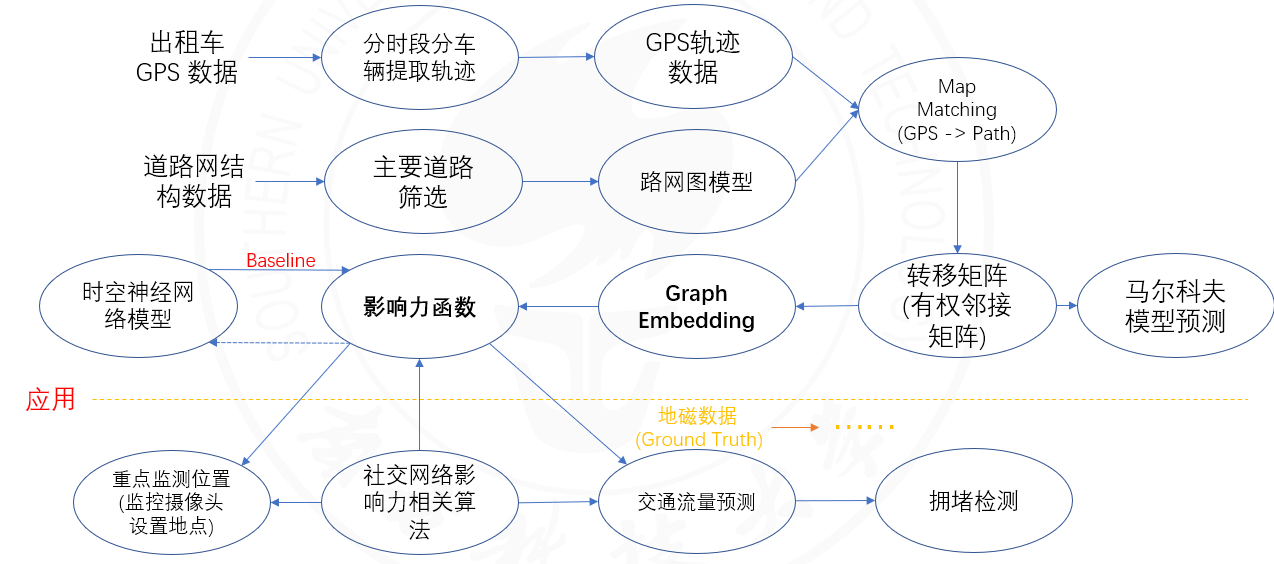
\includegraphics[width=\textwidth]{images/8-1-1.png}
  \caption{System Structure}
  \label{fig: structure}
\end{figure}

\begin{enumerate}
  \item Process taxi GPS data to get tracks
  \item Process road network data to get a basic graph model
  \item Match tracks to each road and get the adjacent matrix of the graph
  \item Try a simple prediction based on Markov model
  \item \textbf{Graph embedding}
  \item \textbf{Influence function design}
  \item Combine spatial-temporal models and use them as baseline
  \item Combine social network influence algorithms to predict traffic network flow, use geomagnetic data as one of the ground truth
  \item Applications: traffic surveillance camera position and traffic jam detection
\end{enumerate}

\subsection{Report Contents}
Breifly, we will state our work in this report as
\begin{itemize}
  \item Transition Matrix and Graph Embedding Analysis by 董正 \& 崔俞崧
  \item Geomagnetic Data Mining 王焕辰
  \item Future Plan by 董正
\end{itemize}

\clearpage
\section{Transition Matrix and Graph Embedding Analysis}
\subsection{Dataset}
\begin{itemize}
  \item Data source: Shenzhen Municipal Government 
  \item Region: Shenzhen
  \item Time: 2019-12-01 to 2019-12-13
  \item Content: Taxi vehicle trajectory data
    \begin{itemize}
      \item License number
      \item Longitude and latitude
      \item Speed
      \item License type
    \end{itemize}
\end{itemize}

\begin{figure}[htb]
  \centering
  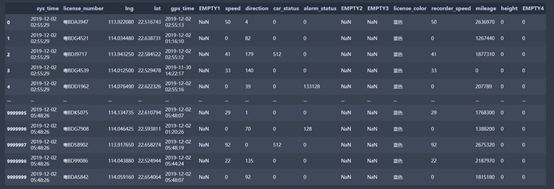
\includegraphics[width=\textwidth]{images/7-2-1.png}
  \caption{Dataset}
  \label{fig: 721}
\end{figure}

\subsection{Transition Matrix}
In the previous period, we did map matching to get taxi trajectory data and a transition matrix.
\begin{itemize}
  \item Size: $16153\times 16153$
  \item Represents the transition probability between adjacent roads
  \item We splited different time intervals in every 3 hours for accuracy
  \item The data we use is from 12.02(Mon.) to 12.07(Sat.), and use 12.08(Sun.) as a test dataset.
\end{itemize}

\clearpage
Next, we gave an flow analysis on this transition matrix:
\begin{figure}[htb]
  \centering
  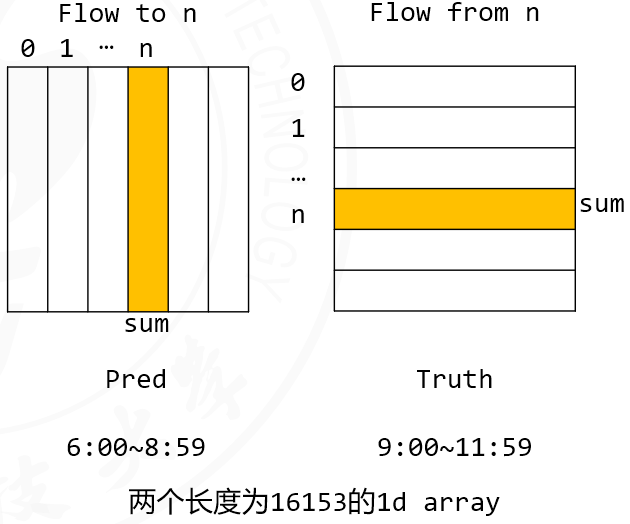
\includegraphics[width=0.8\textwidth]{images/8-2-0.png}
  \caption{Matrix Verification}
  \label{fig: 820}
\end{figure}

Here we choose the 6:00 \textasciitilde 8:59 transition matrix of first 6 days and 9:00 \textasciitilde  11:59 transition matrix of Sunday.
In the left matrix, the sum of column \texttt{n} means how many cars turned to $road_{n}$ (i.e. traffic flow into $road_{n}$) in this time interval.
And in the right matrix, the sum of row \texttt{n} means how many cars turned to other roads from $road_{n}$ (i.e. traffic flow from $road_{n}$).
Therefore, in the ideal situation, these two sum should be fairly close.
\begin{center}
  Flow to $road_n$ in the $(t-1)^{th}$ time interval $\approx$ Flow from $road_n$ in the $t^{th}$ time interval
\end{center}

Expanding it to the whole matrix, we can get an array of sum. Also compute it on test matrix. And we start analysis on these two sum.

\clearpage
After sum on rows and sum on columns, we will get two 1D arrays whose length are 16153.
Then we first calculate their absolute values of difference directly. Remember to divide 6 on the left matrix.
\begin{figure}[htb]
  \centering
  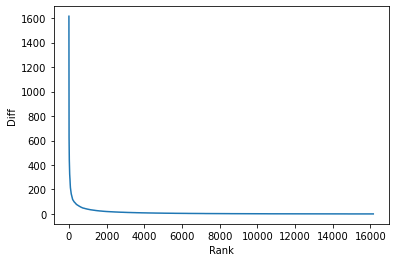
\includegraphics[width=0.7\textwidth]{images/8-2-1.png}
  \caption{Difference of two sum arrays}
  \label{fig: 821}
\end{figure}

From the chart above we can see that some of the roads have a very large difference.
Digging into it a bit we found that it is because we counted self to self (diagonal) in the matrix.
After cleared the diagonal, the differences are:
\begin{figure}[htb]
  \centering
  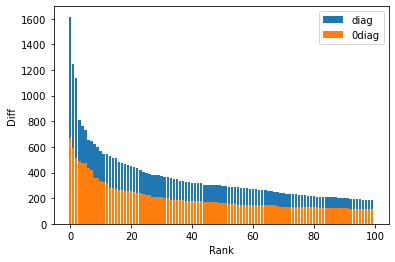
\includegraphics[width=0.7\textwidth]{images/8-2-2.png}
  \caption{Difference of two sum arrays after cleared diagonal}
  \label{fig: 822}
\end{figure}

Still, there are some roads have a large difference. We speculate that this is because we used Sunday as test dataset.
Traffic on holidays has a very different pattern compared to weekdays. Therefore, in the next period, we plan
to try to use Monday to Thursday as train set, and Friday as test set.

\clearpage
\begin{figure}[htb]
  \centering
  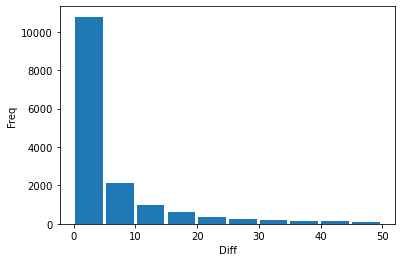
\includegraphics[width=0.7\textwidth]{images/8-2-5.png}
  \caption{Distribution of difference}
  \label{fig: 823}
\end{figure}
The figure above shows the distribution of differences. 
We can see that 97\% of roads is less than 50, and 80\% of roads is less than 10, which indicates
the accuracy of transition matrix.

However, counting differences is not enough. Then we use some metrics to test the error on the whole matrix.
Here we used RMSE, MAE, and MAE/Mean of test matrix. This is because the two transition matrices is very sparse,
i.e. most of them are zeros. Therefore, MAPE cannot be applied because it will divide zero.

We used a controlled experiment. The comparing group calculated errors on same time interval, and both sum on rows.
The results are shown as following:
\begin{figure}[h]
  \centering
  \subfigure[Errors] {
    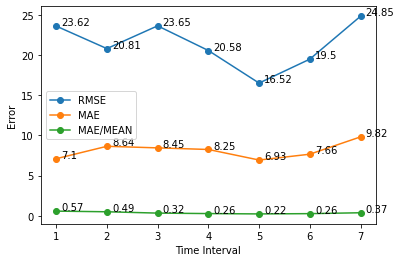
\includegraphics[width=0.45\textwidth]{images/8-2-3.png}
  }
  \quad
  \subfigure[Errors when comparing same time interval] {
    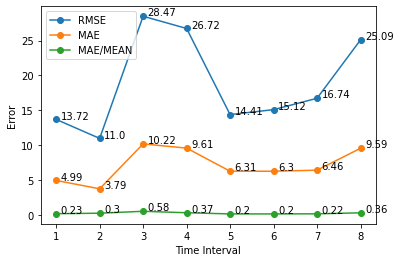
\includegraphics[width=0.45\textwidth]{images/8-2-4.png}
  }
\end{figure}

From the figures above, we can indicate that it is better to use the former time interval to predict the next interval
on rush hours.
However, the performance on night hours is worse than direct prediction. This is because traffic flow is not stable on night hours.
It will increase at the beginning of the day, and decrease at the end of the day.
Direct prediction has a very high error on daytime, which is not acceptable.

\clearpage
\subsection{Graph Embedding}
The most common way to embed a graph is \textit{DeepWalk} with \textit{Word2Vec}.
\begin{figure}[htb]
  \centering
  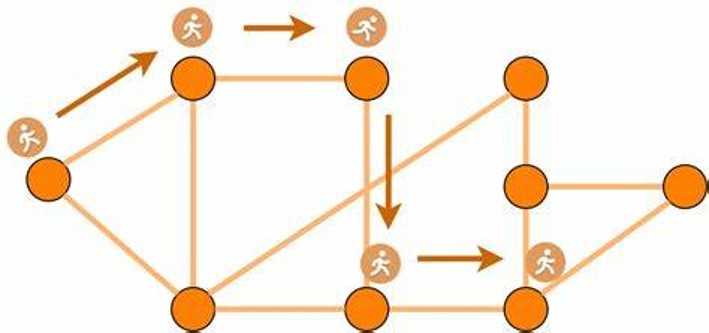
\includegraphics[width=0.8\textwidth]{images/8-2-9.jpg}
  \caption{DeepWalk}
  \label{fig: 829}
\end{figure}

In \textit{DeepWalk} algorithm, we will generate fixed length random path based on the graph model.
Then treat these paths as sentences, use \textit{Word2Vec} technology from NLP to transfrom them to vectors.

However, since map matching gave us a series of taxi trajectories, we can directly apply them to \textit{Word2Vec}.
The advantages are:
\begin{itemize}
  \item Trajectories keeped road connection information.
  \item Trajectories can indicated the transition probability between roads.
  \item No need to set walk length.
  \item Save time, because random walk generation take a lot.
\end{itemize}

What's more, compared to transition matrix, \textit{Word2Vec} can
\begin{itemize}
  \item Represent the transition probability (called similarity) between any two roads.
  \item Have high-dimensional transition information. Because just a 3D transition matrix will be too big to store.
  \item Can deduce influence between roads (next step of our experiment).
\end{itemize}

\clearpage
The figure shows the embedding result on a small dataset, reduced dimension by TSNE algorithm.
\begin{figure}[htb]
  \centering
  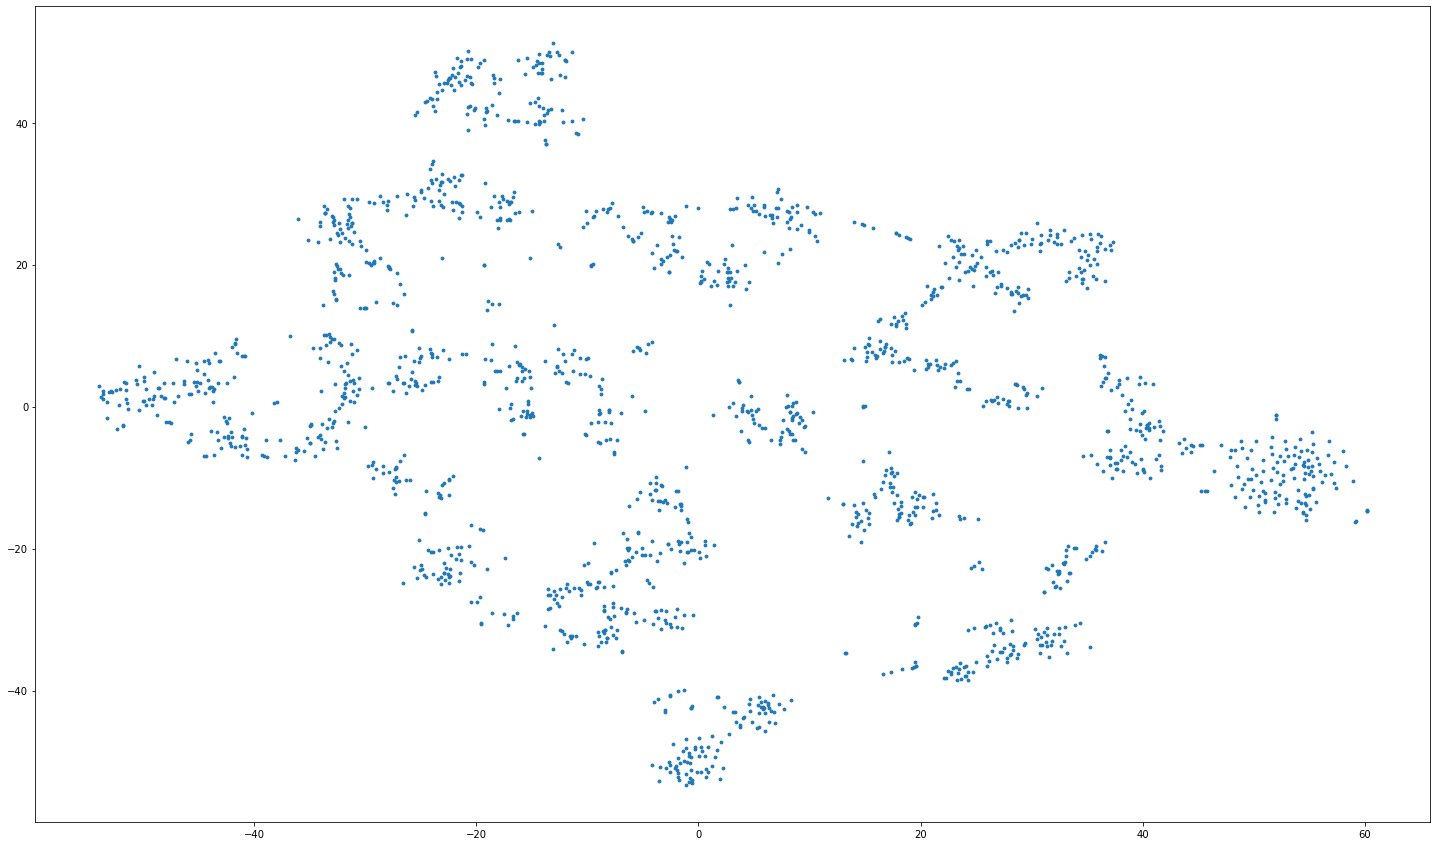
\includegraphics[width=0.8\textwidth]{images/8-2-6.png}
  \caption{Graph Embedding Result After TSNE}
  \label{fig: 826}
\end{figure}

The distance between vectors shows the transition probability between corresponding roads.
From the picture we can tell the road connectivity, since there are obviously many different clusters.

\begin{figure}[h]
  \centering
  \subfigure[Errors] {
    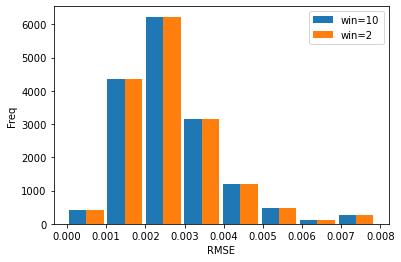
\includegraphics[width=0.45\textwidth]{images/8-2-7.png}
  }
  \quad
  \subfigure[Errors when comparing same time interval] {
    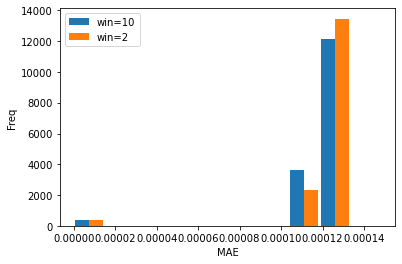
\includegraphics[width=0.45\textwidth]{images/8-2-8.png}
  }
\end{figure}
Then we compare the difference between embedded vectors and transition matrix.
The chart above calculated their RMSE and MAE. First, for each road, devide every element (in transition matrix, it is transition count, and in embedded vectors, they are similarity) by their sum to get a from of probability.
We can know that they have a very small error, which infers that \textit{Word2Vec} keeped the transition probability information in transition matrix.
In addition, it can also represent high-dimensional transition.

In \textit{Word2Vec}, there is a parameter \texttt{window}, which means a word can influence how far in the sentence.
To compare, we set this parameter to 2 (default 10). And the results shows that it had very little effect on embedding.
What's more, it will affect high-dimensional transition, thus, we decided to use default parameters.


\clearpage
\section{Geomagnetic Data Mining}
\subsection{Processing of Geomagnetic Detection Point Drift}
Since observing the position of each detection point by previous results, all points are found to be offset in the same direction.

It is speculated that the base map does not match the coordinate data, so the \textit{coord\_convert} library is used to convert the coordinate data from BD-09 (Baidu coordinate system) to WGS84 (default coordinate system for the map).

After the transformation of coordinates, the coordinates are successfully matched to the corresponding road network on the map, which can be used for the subsequent construction of geomagnetic detection point graph network.
\begin{figure}[htb]
  \centering
  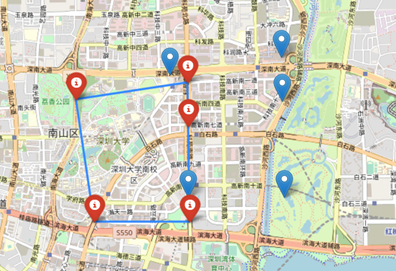
\includegraphics[width=0.8\textwidth]{images/8-3-1.png}
  \caption{Coordinates on the Map before and after Transformation}
  \label{fig: 831}
\end{figure}

\clearpage
\subsection{Vehicle Type Classification}
Using geomagnetic data to provide vehicle types and other features to classify vehicles, and then better used for traffic state, flow prediction

Due to the uneven distribution of the four types of vehicles, the down sampling process is conducted and the available features, such as road, speed and time, are extracted for preliminary classification

SVM and lightgbm were used for classification successively, and the results are as follows. However, the results of both are not ideal because of insufficient features provided by data

\begin{figure}[h]
  \centering
  \subfigure {
    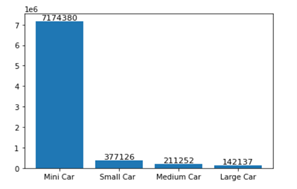
\includegraphics[width=0.45\textwidth]{images/8-3-2.png}
  }
  \quad
  \subfigure {
    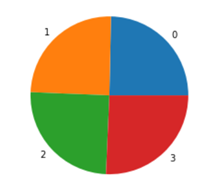
\includegraphics[width=0.45\textwidth]{images/8-3-3.png}
  }
  \caption{The Number of Various Models and the Proportion after Down Sampling}
\end{figure}

\begin{figure}[htb]
  \centering
  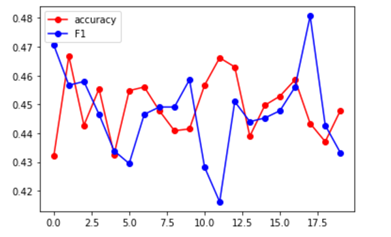
\includegraphics[width=0.8\textwidth]{images/8-3-4.png}
  \caption{Several Scores of Training Results by lightgbm}
  \label{fig: 834}
\end{figure}

\clearpage
\subsection{Traffic Flow Data Further Processing}
In view of the poor effect of vehicle classification and the limitations of geomagnetic data. Therefore, we divide each road vehicle into inflow and outflow according to existing literature and models.

Inspired by the literature, we're going to find out a standard to establish a real graph as far as possible for the unrealistically connected road geomagnetic detection points, and reduce the inflow to outflow error (dividing the map into several districts and construct each graph).

Training only through traffic flow data and graph building through each detection point. As well as predicting traffic flows, it can also serve as a benchmark to evaluate other presented models.

\begin{figure}[htb]
  \centering
  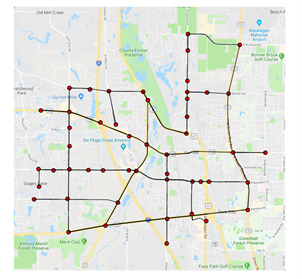
\includegraphics[width=0.5\textwidth]{images/8-3-5.png}
  \caption{Graph of a Community Detection Point}
  \label{fig: 835}
\end{figure}
\begin{figure}[htb]
  \centering
  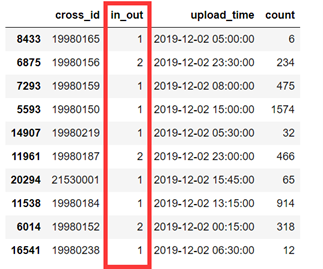
\includegraphics[width=0.5\textwidth]{images/8-3-6.png}
  \caption{Traffic Data after Grouping}
  \label{fig: 836}
\end{figure}

\clearpage
\section{Future Plan}
In the next period, we will learn to use \textit{LibCity} to run baseline algorithms on our model.
\begin{figure}[htb]
  \centering
  
\includegraphics[width=0.7\textwidth]{images/8-4-1.png}
  \caption{LibCity}
  \label{fig: 841}
\end{figure}

From LibCity's GitHub (https://github.com/LibCity/Bigscity-LibCity):

LibCity is a unified, comprehensive, and extensible library, which provides researchers with a credible experimental tool and a convenient development framework in the traffic prediction field. Our library is implemented based on PyTorch and includes all the necessary steps or components related to traffic prediction into a systematic pipeline, allowing researchers to conduct comprehensive experiments. Our library will contribute to the standardization and reproducibility in the field of traffic prediction.

LibCity currently supports the following tasks:
\begin{itemize}
  \item Traffic State Prediction
  \item Traffic Flow Prediction
  \item Traffic Speed Prediction
  \item On-Demand Service Prediction
  \item Origin-destination Matrix Prediction
  \item Traffic Accidents Prediction
  \item Trajectory Next-Location Prediction
  \item Estimated Time of Arrival
  \item Map Matching
  \item Road Network Representation Learning
\end{itemize}

After that, we will start writing paper and also read papers about social network to design our influence function.

% \clearpage
% \phantomsection
% \addcontentsline{toc}{section}{References}
% \bibliographystyle{ieeetr}
% \bibliography{references}

\end{document}